\section{Conclusions}
% Original presentation frame 22
\begin{frame}[t,shrink=5]{Structured operator support is promising, while representation and uncertainty remain the main limits}
\begin{columns}[T,onlytextwidth]
\begin{column}{0.49\textwidth}
\begin{block}{Key messages from the 6D surrogate study}
\begin{itemize}
\item Collective effects motivate surrogate modelling of distribution evolution.
\item The FNO connects reduced longitudinal dynamics with spectral wake response.
\item In the full-lattice endpoint task, local attention and graph-kernel propagation improve over dense causal mixing in the selected runs.
\end{itemize}
\end{block}

\end{column}
\begin{column}{0.49\textwidth}
\begin{block}{Conditions on those conclusions}
\begin{itemize}
\item The model is bound by the sampled parameter domain,
\item The 15 projections are not a unique 6D reconstruction,
\item The latent ensemble is not calibrated predictive uncertainty,
\item Intermediate dynamics and omitted physical effects require new simulation data.
\end{itemize}
\end{block}
\begin{alertblock}{Next step}
A broader, checkpointed and uncertainty-calibrated FCC-ee HEB surrogate.
\end{alertblock}

\end{column}
\end{columns}

\sources{\parencite{ghribi2026updates}.}

\end{frame}

% Original presentation frame 23
\begin{frame}[t,shrink=5]{The complete 6D result is traceable to public code, fixed data splits and archived machine inputs}
\begin{columns}[T,onlytextwidth]
\begin{column}{0.49\textwidth}
\begin{block}{Public outputs}
\begin{itemize}
\item \href{https://github.com/SantiagoM1227/ML4CollEffects}{ML4CollEffects GitHub repository},
\item Zenodo dataset, DOI \href{https://doi.org/10.5281/zenodo.21644178}{10.5281/zenodo.21644178},
\item IPAC'26 paper MOP1072.
\end{itemize}
\end{block}

\end{column}
\begin{column}{0.49\textwidth}
\begin{block}{Contribution beyond the preliminary paper}
Full CVAE formulation and latent diagnostics, global/local Transformer comparison, graph-kernel interpretation, GNO benchmark, physical-statistics head, conditional latent uncertainty, under-dispersion diagnosis, explicit limitations and reproducibility record.
\end{block}

\end{column}
\end{columns}

\sources{\parencite{ghribi2026updates,martinez2026code,martinez2026dataset}.}

\end{frame}

% Original presentation frame 24
\begin{frame}[plain]
\begin{center}{\LARGE Thank you}\par\bigskip\begin{columns}[T,onlytextwidth]
\begin{column}{0.49\textwidth}
\begin{center}
\includegraphics[width=\linewidth,height=40mm,keepaspectratio]{thank_you_character_left.png}\end{center}
\end{column}
\begin{column}{0.49\textwidth}
\begin{center}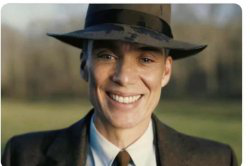
\includegraphics[width=\linewidth,height=40mm,keepaspectratio]{thank_you_character_right.png}\end{center}
\end{column}
\end{columns}
{\large Questions?}\end{center}
\end{frame}

